\documentclass[dcc,uchile]{fcfmcourse}
\usepackage{teoria}
\usepackage[utf8x]{inputenc}
\usepackage{amsmath}
\usepackage{amsfonts,setspace}
\usepackage{caption}
\usepackage{listings}
\usepackage{hyperref}
\usepackage{color}
\usepackage{soul}
\usepackage{emojis}
\usepackage[spanish]{babel}
\usepackage[lined,boxed,commentsnumbered]{algorithm2e}
\SetKwInput{KwIn}{Input}
\renewcommand{\algorithmcfname}{Algoritmo}
\renewcommand{\figurename}{Figura}
\renewcommand{\tablename}{Tabla}


\definecolor{pblue}{rgb}{0.13,0.13,1}
\definecolor{pgreen}{rgb}{0,0.5,0}
\definecolor{porange}{rgb}{0.9,0.5,0}
\definecolor{pgrey}{rgb}{0.46,0.45,0.48}

\lstset{language=Java,
  showspaces=false,
  showtabs=false,
  breaklines=true,
  showstringspaces=false,
  breakatwhitespace=true,
  commentstyle=\color{porange},
  keywordstyle=\color{pblue},
  stringstyle=\color{pgreen},
  basicstyle=\ttfamily,
  moredelim=[il][\textcolor{pgrey}]{$ $},
  moredelim=[is][\textcolor{pgrey}]{\%\%}{\%\%}
}

\newenvironment{codebox} {\small \ttfamily \obeylines \begingroup \setstretch{-2.4}} {\endgroup}

% COmpletar titulo
\title{Tarea 1 - R-Trees}
\course[CC4102]{Diseño y Análisis de Algoritmos}
\professor{Gonzalo Navarro}
\assistant{Manuel Cáceres}
\assistantt{Jaime Salas}
\assistantt{Tomás Perry}

\begin{document}
\captionsetup[table]{name=Tabla}
\captionsetup[table]{name=Figura}

\maketitle
\vspace{-1ex}
\section{Introducción}
Un R-tree es un árbol, parecido al B-tree, que permite manipular \textit{rectángulos} en memoria secundaria. Se permite \textit{insertar} rectángulos y \textit{buscar} rectángulos. La operación de búsqueda es como sigue: Dado un rectángulo $C$ como entrada, debemos retornar todos los rectángulos en el R-tree que intersectan $C$.

El objetivo de esta tarea es implementar y evaluar en la práctica diferentes heurísticas para la implementación de un R-tree. En particular, nos interesa analizar el impacto de variantes de inserción sobre la operación de búsqueda. Para la evaluación consideremos datos sintéticos y reales. Se espera que se implementen los algoritmos y se entregue un informe que indique claramente los siguientes puntos:

\begin{enumerate}[1.]
    \item Las \textit{hipótesis} escogidas antes de realizar los experimentos.
    \item El \textit{diseño experimental}, incluyendo los detalles de la implementación de los algoritmos, la generación de las instancias y las medidas de rendimiento utilizadas.
    \item La \textit{presentación de los resultados} en forma de una descripción textual, tablas y/o gráficos.
    \item El \textit{análisis e interpretación} de los resultados.
\end{enumerate}
\section{Las Estructuras}
Un R-tree cumple los siguientes \textit{invariantes}, similares a las de un B-tree:
\begin{enumerate}[1.]
    \item Cada nodo interno representa conceptualmente un rectángulo: el \textit{Minimum Bounding Rectangle} (MBR) de los rectángulos de los nodos que cuelgan de él\footnote{El rectángulo más pequeño que contiene a todos estos rectángulos.}. De esta forma, al hablar de un nodo también hablamos de un rectángulo.
    \item Los rectángulos correspondientes a datos se encuentran almacenados en las hojas del árbol. Estos nodos también almacenan/representan el MBR de esos rectángulos.
    \item Cada nodo de un R-tree almacena \textit{físicamente} al menos $m$ rectángulos y a lo más $M$ rectángulos (correspondientes a los MBRs de sus hijos 0, en el caso de las hojas, a los datos representados), a excepción de la raíz que debe almacenar $2$ rectángulos.
    \item Todos los nodos hojas están a la misma profundidad en el árbol.
\end{enumerate}
\begin{figure}[h]
    \centering
    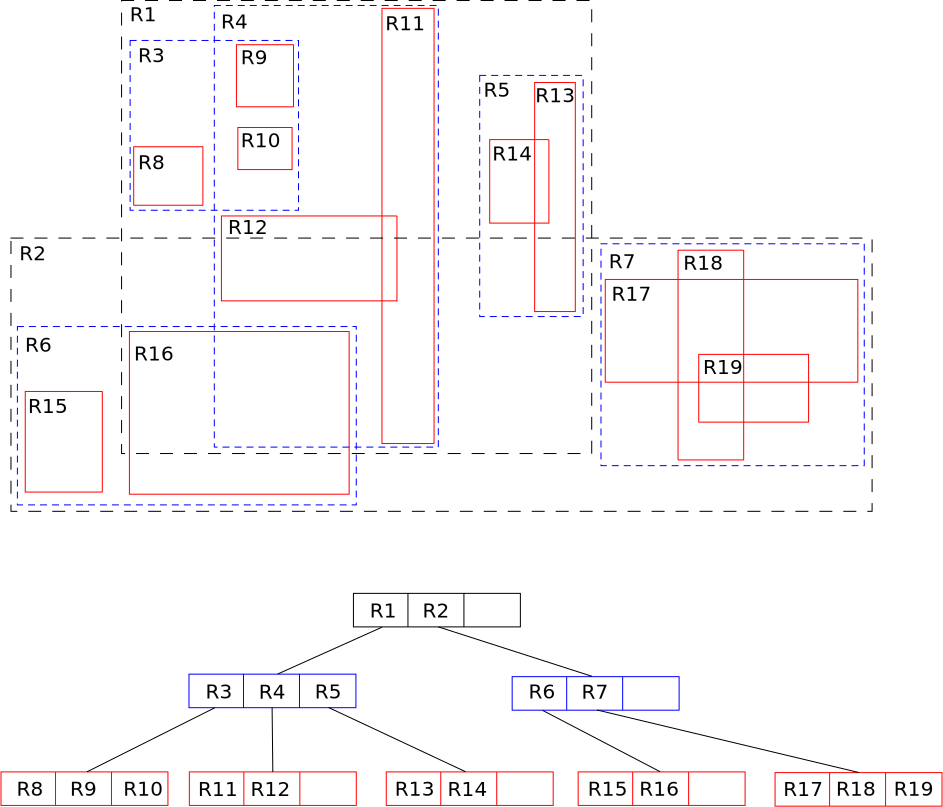
\includegraphics[scale=0.5]{imagenes/R-tree}
    \caption{Ejemplo de R-tree}
    \label{fig:my_label}
\end{figure}
\subsection{Buscar}
Dado un rectángulo $C$, la operación de búsqueda recorre el árbol para encontrar todos los rectángulos en los nodos hojas que lo intersectan. Si en algún nodo interno, un MBR no intersecta a $C$, se puede descartar el subárbol correspondiente.
\subsection{Insertar}
Dado un rectángulo $C$, la operación de inserción recorre el árbol desde la raíz hasta alguna hoja, e inserta $C$ en esa hoja, modificando el árbol para preservar los invariantes.

El recorrido para la inserción se realiza de la siguiente forma:
\begin{itemize}
    \item Si los hijos del nodo actual son hojas se escoge una hoja y se inserta $C$ en ésta, terminando el recorrido.
    \item En caso de que los hijos del nodo actual no sean hojas, se escoge el MBR que deba crecer lo menos posible para incluir el nuevo dato, y se desciende por el subárbol correspondiente.
    \item Para el descenso en el árbol, si los MBRs deben crecer lo mismo para albergar el nuevo nodom se baja por el MBR que tenga la menor área. En caso de empate, se elige uno al azar.
\end{itemize}
Una vez insertado $C$, es necesario reestablecer los invariantes que se puedan haber roto.
\begin{itemize}
    \item Si un nodo queda con más de $M$ rectángulos en él, se produce un \textit{oerflow} que rompe el invariante 3. Hay múltiples formas de tratar esto, como se verá más adelante: cada una de estas formas puede pasar a llevar otros invariantes y deben hacerse cargo de ésto.
    \item Es necesario actualizar los MBRs desde la hoja hacia la raíz, para recuperar el invariante 1.
\end{itemize}
\subsection{Manejo de overflows}
Supongamos que tenemos un nodo con $M+1$ rectángulos. El cómo solucionar esta situación y restablecer el invariante 3 no es directo. Por ejemplo, si intentamos dividir el nodo en dos, no es claro cuáles rectángulos debieran quedar en cada uno (¡computar una redistribución ``ideal'' tomaría tiempo exponencial!). En general, se usan heurísticas, lo que significa que podemos tener múltiples variantes del R-tree. Las heurísticas que utilizaremos dividen el nodo en dos: es importante notar que después de definir ambos nodos, es necesario computar el MBR de los rectángulos que quedan en cada uno de éstos.

Cada heurística que se muestra tiene la siguiente estructura:
\begin{itemize}
    \item Se divide el nodo con overflow en dos, según la heurística. Se computa el MBR de cada uno y se almacena en el nodo.
    \item Se reemplaza el nodo con overflow por los dos nodos nuevos en su padre, actualizando el MBR.
    \item Como se agregó un nodo extra al padre, puede sufrir overflow, caso en el que se repite el algoritmo ``hacia arriba''.
    \item Si la raíz sufre overflow, se crea una nueva raíz con dos nodos hijos.
\end{itemize}
\subsubsection{LinearSplit}
Se eligen los dos rectángulos más alejados como miembros iniciales (y MBR) de cada nuevo nodo, respectivamente. Para determinar esto, se realiza lo siguiente para cada dimensión de los datos:
\begin{itemize}
    \item Para cada dimensión, se determina el rectángulo con el valor máximo del lado ``bajo'' (ej. aquel cuyo lado izquierdo está más a la derecha) y aquel con el valor mínimo del lado ``alto'' (ej. aquel cuyo lado derecho está más a la izquierda). Se almacena la separación entre estos lados.
    \item Cada separación se normaliza dividiendo por el rango del conjunto de rectángulos en la dimensión correspondiente.
    \item Se selecciona el par que tenga la mayor separación normalizada en alguna de las dimensiones.
\end{itemize}
Una vez que los rectángulos iniciales de cada nodo han sido escogidos, se toma cada rectángulo restante (en orden aleatorio) y se agrega al nodo cuyo MBR experimente el menor incremento en área; luego se recomputa el MBR del nodo. Debe tener cuidado para asegurar que los dos nuevos nodos temrinan con al menor $m$ MBRs.
\subsubsection{QuadraticSplit}
Se eligen los dos rectángulos tales que el MBR del par tiene el área inútil más grande (definida como el área del MBR menos el área de cada rectángulo) como miembros iniciales de los nuevos nodos (en caso de empates puede elegirlos arbitrariamente).

Una vez que los rectángulos iniciales de cada nodo han sido escogidos, se procede como en la estrategia anterior.

Al momento de repartir los MBRs entre los dos nuevos MBRs, tanto en LinearSplit como en QUadraticSplit, rompa el empate entre los candidatos escogiendo el que tenga menor área total, seguido del que tenga menor número de MBRs asignados, y si sigue el empate escoja uno arbitrariamente.
\subsubsection{Greene's Split}
En un primer paso se determinan los dos rectángulos más distantes, siguiento los pasos de LinearSplit. Luego:
\begin{itemize}
    \item Se define la \textit{dirección de corte} como el eje perpendicular a la dimensión que tenía la mayor separación normalizada (resolver empates arbitrariamente).
    \item Los $M+1$ rectángulos se ordenan por valor mínimo a lo largo del eje (ej. si el eje es el horizontal, se ordenan por la coordenada del lado izquierdo).
    \item Los primeros $M/2-1$ rectángulos quedan en el primer nodo, mientras que los restantes quedan en el segundo.
\end{itemize}
\subsubsection{Heurística inspirada en $R^*$-tree}
Una estrategia usada en una variante de R-trees denominada $R^*$-trees\footnote{Los $R^*$-trees combinan esta estrategia de división de nodos con una estrategia de reinserción, que no incluiremos en esta tarea. Además, alteran la forma de bajar en el árbol para la inserción.} se lleva a cabo como sigue.

En primer lugar, se define el \textit{margen} (para seguir la nomenclatura de la literatura) de un rectángulo como su perímetro. Por otro lado, es necesario definir lo que será una \textit{distribución} del conjunto de rectángulos. Suponiendo que se tienen $M+1$ rectángulos ordenados en una lista llamaremos distribución a dividir la lista en dos conjuntos no vacíos: el de los $m+k$ primeros y el de los restantes, dado un parámetro $k\in[0,M+1-2m]$. Así, hay $M+2-2m$ distribuciones posibles.

En el primer paso del split, se escoge la dimensión de corte. Se ordenan, para cada dimensión, los rectángulos por sus valores mínimos a lo largo de ésta. Luego, para cada distribución (es decir, para cada posible valor de $k$), se calcula la suma del margen del MBR de cada uno de los dos grupos generados. Se calcula la suma total $S$ de estos márgenes para todas las distribuciones posibles dado $k$. Se repite el proceso ordenando según los valores máximos. Finalmente, se escoge la dimensión que tenga el mínimo valor $S$.

En un segundo paso, se escoge el índice de corte a lo largo de la dimensión elegida. Para esto, se elige la distribución (o sea, el valor $k$) que produzca la mínima intersección entre los MBRs que engloban a cada uno de los dos grupos de la distribución. En caso de empate, se escoge la distribución que genere los MBRs de menor área. De continuar el empate divida los elementos en conjuntos del mismo tamaño ($\pm1$ si $M+1$ es impar).
\section{Implementación}
Implemente dos versiones de la estructura, utilizando dos de las heurísticas presentadas para el overflow. Si lo desea, puede proponer e implementar una heurística propia (explicando claramente en su informe cómo funciona y cuidando que preserve los invariantes de la estructura) e implementarla, junto con una de las especificadas en la sección anterior.
\section{Experimentos}
Escoja el parámetro $M$ de acuerdo a las características de su máquina de manera que un nodo quepa siempre en una página de disco. Documente las características de su máquina, el sistema operativo, lenguaje y compilador utilizados, RAM, y características del disco duro. Utilice $m=40\%$ de $M$ para el split.

En los experimentos se pide comparar 1. el tiempo de la construcción del R-tree con cada variante de insertar, 2. el espacio ocupado y porcentaje de llenado de las páginas de disco y 3. evaluar el desempeño de la operación \textit{buscar}.
Use datos sintéticos y opcionalmente reales. Genere conjuntos de $n$ rectángulos con $n\in \{2^9,\ldots,2^25\}$. Deberá generar los rectángulos al azar de la siguiente manera: las coordenadas de uno de los vértices deben ser reales uniformemente distribuidos en el rango $[1,100]$. En este enlace \href{https://www.census.gov/geo/maps-data/data/tiger.html}{https://www.census.gov/geo/maps-data/data/tiger.html} puede encontrar un dataset real de MBRs, o también puede usar otro que este públicamente disponible; debe documentar las características del dataset real usado (descripción, formato, tamaño, distribución de las coordenadas y áreas de los MBRs, etc.).

Se considerará \textit{0.5 puntos extra} si también hace uso de algún dataset real.

Para cada dataset de tamaño $n$, construya el R-tree con las dos variantes. Una vez construido el R-tree, genere $n/10$ rectángulos al azar para hacer las consultas de búsqueda. Documente en cada caso el tiempo y cantidad de accesos a disco promedio de búsqueda.
\subsection{Opcional}
Esta parte se considerará como 1 punto extra sobre la nota de la tarea. Comparar sus implementaciones con un R-tree estable, repitiendo la metodología anterior:
\begin{itemize}
    \item Usando solo la RAM como almacenamiento compare su estructura versus la implementación de R-tree de \texttt{boost}: \href{http://www.boost.org/doc/libs/1_62_0/libs/geometry/doc/html/geometry/spatial_indexes.html}{http://www.boost.org/doc/libs/1_62_0/libs/geometry/doc/html/geometry/spatial_indexes.html}, o
    \item Usando disco como almacenamiento, compare su estructura con el R-tree disponible en alguna base de datos como PostgreSQL o SQLite.
\end{itemize}
\section{Entrega de la Tarea}
\begin{itemize}
    \item La tarea puede realizarse en grupos de a lo más 3 personas.
    \item Para la implementación puede utilizar C, C++ o Java. Para el informe se recomienda utilizar \LaTeX .
    \item Siga buenas prácticas (\textit{good coding practices}) en sus implementaciones.
    \item Escriba un informe claro y conciso. Las ponderaciones del informe y la implementación en su nota final son las mismas.
    \item Tenga en cuenta las sugerencias realizadas en las primeras clases sobre la forma de realizar y presentar experimentos.
    \item La entrega será a través de U-Cursos y deberá incluir el informe junto con el código fuente de la implementación (y todas las indicaciones necesarias para su ejecución).
    \item Se permiten atrasos con un descuento de 1 punto por día.
\end{itemize}
\section{Links}
\begin{itemize}
    \item El paper original de los R-trees: \href{http://www-db.deis.unibo.it/courses/SI-LS/papers/Gut84.pdf}{http://www-db.deis.unibo.it/courses/SI-LS/papers/Gut84.pdf} 
\end{itemize}


\end{document}

